%!TEX root = pset1.tex

\section{Ridge Regression}\label{sec:ridge_reg}
\subsection{Implementation}
Ridge regression is the particular case of regularized least squares with a quadratic regularizer term.  The error function that we aim to minimize over is given by:
\begin{equation} \label{eq:ridge_error_fn}
\frac{1}{2} \sum_{n=1}^{N} (t_n - \M{w}^T \phi (\M{x}_n) )^2 + \frac{\lambda}{2} \M{w}^T \M{w}
\end{equation}

The closed-form solution of this problem is well-known, and can be derived by setting the gradient of (\ref{eq:ridge_error_fn}) equal to zero.  The optimal solution for $\M{w}$ is provided by Bishop (2006), page 145:

\begin{equation} \label{eq:ridge_sol}
\M{w}_{ridge} = (\lambda \M{I} + \Phi^T \Phi)^{-1} \Phi^T \M{t}
\end{equation}

We coded this method in MATLAB and tested our program using data from Bishop Figure 1.4, varying the parameters of $\lambda$ and $M$.  For the extreme cases, we observed that if $\lambda \leq 0.0001$, then $\M{w}_{ridge} \approx \M{w}_{OLS}$, and if $\lambda \geq 100$, then $\M{w}_{ridge} \approx \M{0}$.  If $M = 1$, then the ridge regression prediction is linear, and as $M$ increases, our prediction curves to fit the training data more closely.  Predictions resulting from different choices of the parameters $\lambda$ and $M$ are shown in Figure~\ref{fig:ridge_plots}.  

\begin{figure}[h!]
\centering
    \begin{subfigure}[b]{0.4\textwidth}
	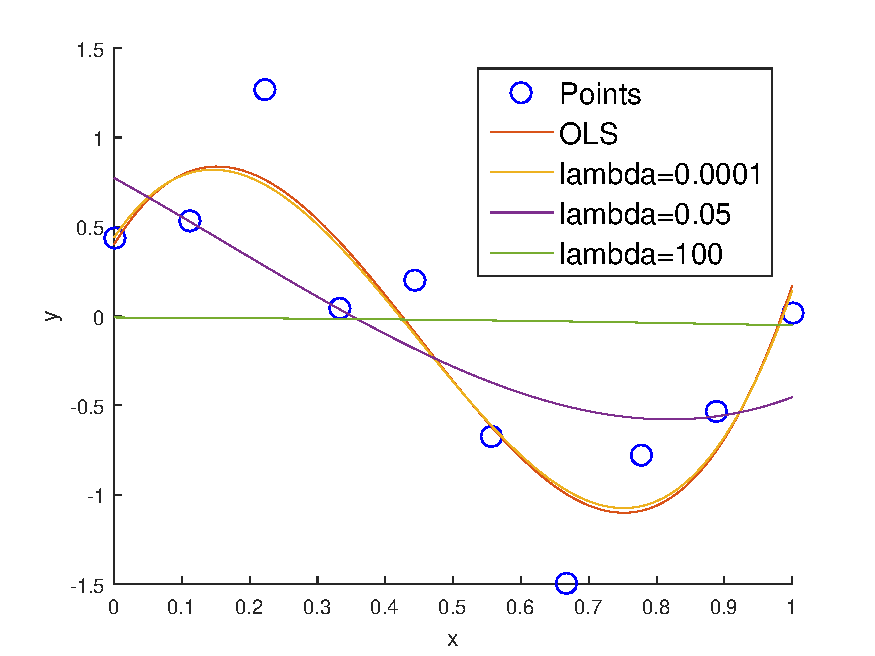
\includegraphics[scale=0.5]{hw1_3_1a.pdf}
	\caption{$M$ = 3 fixed, vary $\lambda$}
    \end{subfigure}
    \quad\quad\quad\quad\quad
    \begin{subfigure}[b]{0.4\textwidth}
	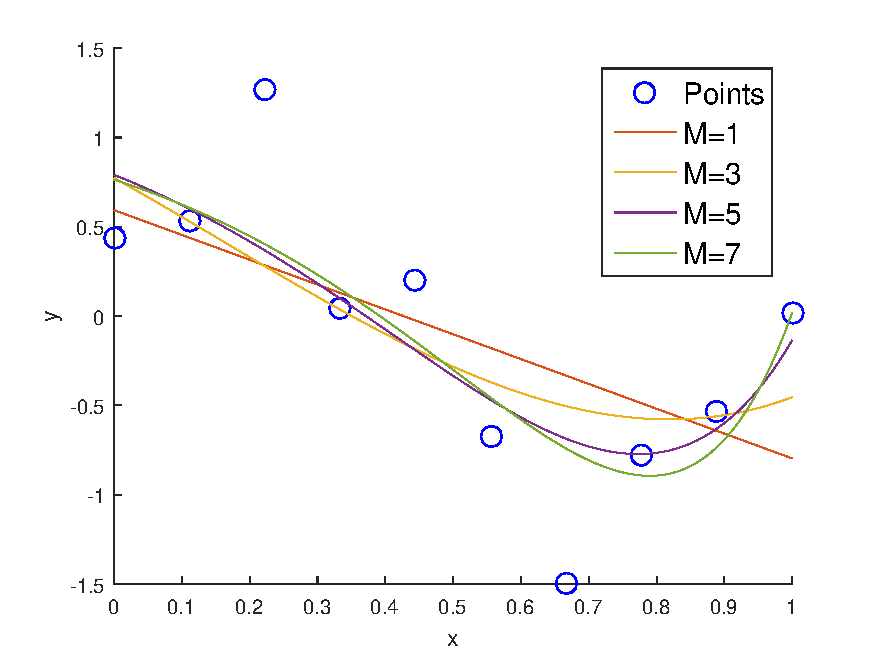
\includegraphics[scale=0.5]{hw1_3_1b.pdf}
	\caption{$\lambda$ = 0.05 fixed, vary $M$}
    \end{subfigure}
    \hfill
\caption{Prediction curves from ridge regression using data from Bishop 1.4.  $M$ = order of polynomial basis function, $\lambda$ = regularization parameter.} \label{fig:ridge_plots}
\end{figure}

\subsection{Model Selection}
To optimize parameter values for $\lambda$ and $M$, we build our models using training data and then compare out-of-sample performance on validation data.  For this example, we performed a grid search over the ranges: $\log_{10}(\lambda) = \{-10,\ldots,10\}$, $M = \{0,\ldots, 9\}$.  We found that the model with $\lambda = 1$ and $M = 4$ yields the lowest MSE on validation data, so we select these to be the final parameter values.  This model leads to MSE = 0.1056 on the validation data and MSE = 2.6988 on the test data.  

In general, we observe that models with relatively low MSE on the validation set tend to have relatively low MSE on the test set.  Heat maps of the MSE values for different parameter values are shown in Figure~\ref{fig:heat_map}.   As expected, test MSE is higher on average, and the plots are similar for most parameter values.  Discrepancies between the heat maps may be attributed to the prescence of an outlier in the training set.  In both heat maps, we see that the top right corner (high M, low $\lambda$), which corresponds to complex models with little regularization, lead to the worst performance on out-of-sample data.  

\begin{figure}[htbp]
    \begin{subfigure}[b]{0.4\textwidth}
	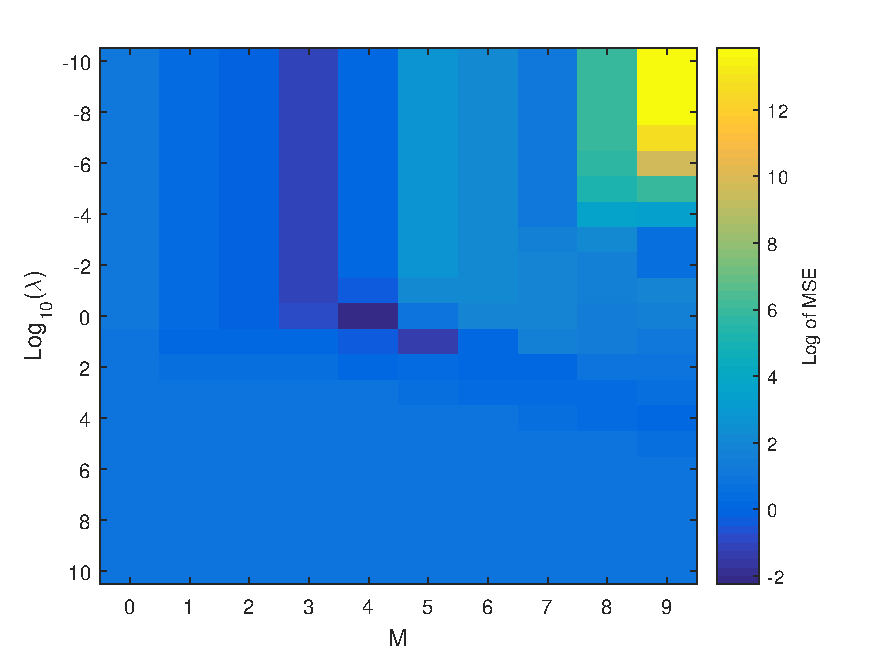
\includegraphics[scale=0.5]{hw1_3_2.pdf}
	\caption{Validation MSE}
    \end{subfigure}
    \quad\quad\quad\quad\quad\quad
    \begin{subfigure}[b]{0.4\textwidth}
	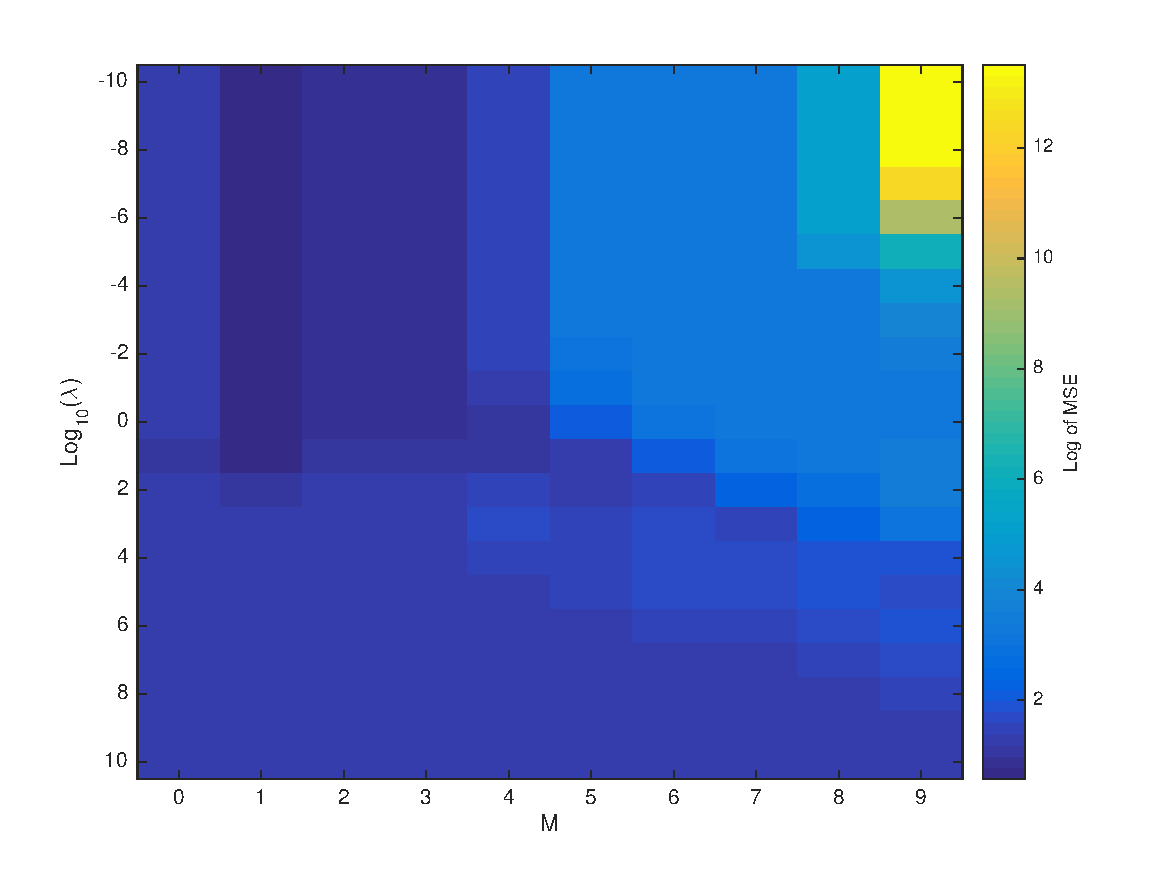
\includegraphics[scale=0.5]{hw1_3_2b.pdf}
	\caption{Test MSE}
    \end{subfigure}
\caption{Heat map of the MSE for ridge regression on the validation and test sets, varying the parameters $M$ and $\lambda$.  Color gradient from low MSE (navy blue) to high MSE (yellow).} \label{fig:heat_map}
\end{figure}

\subsection{BlogFeedback Dataset}
To test our ridge regression algorithm in a real-world application, we apply our method to the BlogFeedback regression problem from Krisztian Buza at the Budapest University.  In the dataset, a blog post is described by 280 features, and our goal is to predict the number of comments it will receive in the next 24 hours.  We are given a training, validation, and test set of blog post observations, and assume a simple linear basis function for this problem.  

Doing a line search over the range $\log_{10}(\lambda) = \{-4,\ldots,10\}$, we find that $\lambda = 10,000$ yields the lowest MSE on validation data.  This model leads to MSE = 1014.4 on the validation data and MSE = 894.36 on the test data.  